\documentclass{article}
\usepackage[minionint,mathlf,textlf]{MinionPro} % To gussy up a bit
\usepackage[margin=1in]{geometry}
\usepackage{graphicx} % For .eps inclusion
%\usepackage{indentfirst} % Controls indentation
\usepackage[compact]{titlesec} % For regulating spacing before section titles
\usepackage{adjustbox} % For vertically-aligned side-by-side minipages
\usepackage{array, mathrsfs, mhchem, amsmath} % For centering of tabulars with text-wrapping columns
\usepackage{hyper ref}
\usepackage[autolinebreaks,framed,numbered]{mcode}
\pagenumbering{gobble} 
\setlength\parindent{0 cm}
\begin{document}
\large

\section*{Recap from last time}
\begin{itemize}
\item Prior to the break, we discussed natural biological oscillators and clocks, and the features of those systems that impart regularity in period, amplitude, and synchronicity.
\item We discussed two basic system topologies associated with smooth vs. relaxation oscillators, and the consequences of the two timescales of relaxation oscillators for phase stability following perturbation.
\item We introduced the notion that the transcriptional feedback loop of the cyanobacterial clock may stabilize the underlying post-translational oscillator by regulating the stoichiometry of KaiA vs. KaiBC; you will discuss this further in section on Friday.
\item We saw that coupling, e.g. through an extracellular signal, can phase lock oscillations in multiple organisms (\textit{Dicty}, Japanese tree frogs) and even link oscillators that have different intrinsic phases (fireflies).
\item We also briefly mentioned robustness to external conditions such as division time and temperature (more on the latter in a moment).
\item During today's lecture, we'll focus on synthetic biological oscillators. Attempting to recreate the features mentioned above reveals something about their relative efficacy which is complementary to the analytical, simulation-based, and experimental approaches we have seen over the last few days, and which will motivate our transition into stochastic models on Wednesday.
\end{itemize}

\section*{Temperature compensation}

\begin{itemize}
\item During our last lecture, a student asked which properties of the cyanobacterial clock make its period robust to changes in temperature. I speculated that the reversibility of each step in the clock was to blame: that both reaction rates scaled similarly and therefore cancelled out.
\item This argument, which apparently was originally proposed by our recently-departed Woody Hastings (Hastings and Sweeney, 1957) in the context of a dinoflagellate circadian rhythm, appears not to hold for the cyanobacterial clock where the phosphorylation and dephosphorylation reactions have very different activation energies\footnote{The concept does seem effective for the circadian clock of \textit{Arabidopsis}; see Gould et al., 2006.}. However, natural and synthetic temperature compensation have been the subject of a few recent studies which I was unaware of at that time but may interest you, as they suggest relatively general mechanisms for achieving temperature robustness.
\item As I mentioned then, most reactions have temperature-dependent rates that follow the Arrhenius rate law:
\[ k_{\textrm{cat}} \sim e^{-E_a / k_bT} \]
Biologists often refer to the activation energy $E_a$ as $\Delta G^{\ddag}$.
\item Most biological reactions are occurring somewhere near 25$^o$C, and many enzyme-catalyzed reactions have an empirically-determined activation energy in the ballpark of 50 kJ/mol. With these values, for every 10 degrees that the temperature increases, the reaction rate approximately doubles.
\item For the cyanobacterial system, the model given by Rust et al. (2007, 2011) successfully assumed first-order kinetics, so let's suppose that overall the rate of product accumulation looks something like:
\[ \frac{dP}{dt} = k_{\textrm{cat}} \left[ E \right] \sim \left[ E \right] e^{-E_a / k_bT} \]
where $[E]$ is the concentration of the enzyme.
\item Now, imagine that a single enzyme catalyzes many of the reactions needed for clock cycle progression. We know this is the case for KaiC in the cyanobacterial clock. One of the reactions will have a higher activation energy than the others and be rate-limiting for the clock's progression.
\item If the enzyme concentration and temperature are low enough, then the substrate of the rate-limiting reaction will begin to accumulate. Since these substrates bind the enzyme at the same active site as the others, they become competitive inhibitors of the other reactions which the enzyme would catalyze. This slows down progression of the clock as a whole.
\item This idea was treated analytically by Hatakeyama and Kaneko in 2012, who accounted for specifics of the cyanobacterial KaiAC system and found it to maintain a relatively constant period over a large range of temperatures. Contrary to what I speculated last time, the reversibility of each step does \textit{not} appear to be important for the temperature compensation and in fact the activation energies for phosphorylation and dephosphorylation are very different, so that we cannot consider the rates to scale equally as temperature varies. This difference in activation energies is indeed important in their model.
\item Later in this lecture, we'll see how this principle can be employed to improve synchronization of a synthetic clock.
\end{itemize}

\section*{Introduction to the Hasty group's synthetic oscillators}
\begin{itemize}
\item We have already mentioned the repressilator in class, and indeed there are many groups doing important work on synthetic oscillators which we might have highlighted in this lecture. However, an appealing option is to study the various improvements made by one lab to a baseline system. In this way, we avoid comparing apples to oranges and gain as much benefit as possible from the synthetic approach.
\item Jeff Hasty's group at UCSD has been considering variations on a synthetic relaxation oscillator, both analytically and experimentally, since the mid-aughts in an extraordinary succession of Nature, Science, and PRL papers. The original topology of this oscillator (Stricker et al., 2008) is shown below:
\end{itemize}
\begin{center}
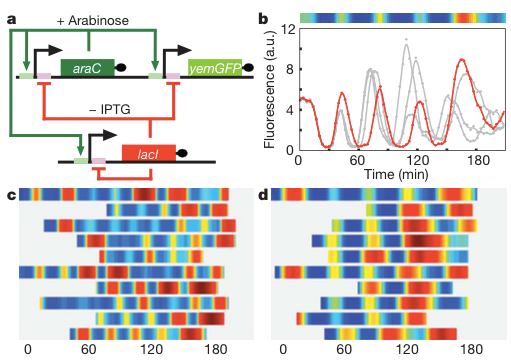
\includegraphics[width=0.6\textwidth]{stricker_trace.png}
\end{center}
\begin{itemize}
\item One feature, indicated by the black tags in the figure, is the inclusion of LAA tags on each protein. These are the short peptide sequences that target, e.g., peptides from stalled ribosomes for proteolysis in \textit{E. coli}. They were intended in this context to increase the turnover rates so that the period of the clock would not be limited by dilution due to cell division. However, as we will see later, they can also be used to couple protein levels through shared degradation machinery.
\item Time courses of individual cells containing the original circuit reveal variability in amplitude and period, not dissimilar from the results for a simple negative autoregulatory circuit:
\end{itemize}
\begin{center}
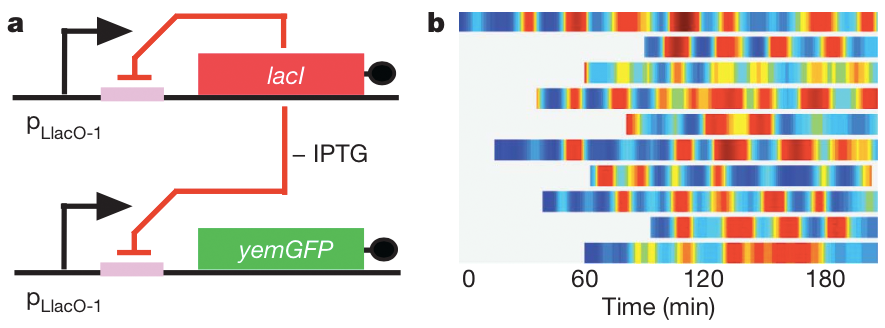
\includegraphics[width=0.6\textwidth]{stricker_negreg.png}
\end{center}
\begin{itemize}
\item The consistency in period and amplitude evident in these traces leaves some room for improvement by the bells and whistles we have introduced so far. 
\end{itemize}

\section*{Temperature compensation (Hussain et al.)}
\begin{itemize}
\item  The original oscillator does not display temperature compensation: the period of the clock decreases as one would expect from reactions following Arrhenius rate laws.  At first blush, the Hasty lab oscillator would not seem to be a good candidate for temperature compensation. Many of the rates are set by transcriptional and translational machinery which we do not want to dicker with or overload (e.g. to synchronize using the method elaborated by Hatakeyama and Kaneko).
\item Hussain et al. (2014) introduce temperature compensation into this oscillator by using a temperature-sensitive variant of LacI. The probability of this repressor misfolding/becoming nonfunctional increases with temperature. More of the repressor needs to build up before promoters in this system are repressed: as a result, temperature-sensitive LacI tends to increase the period of the clock as temperature rises.
\end{itemize}
\begin{center}
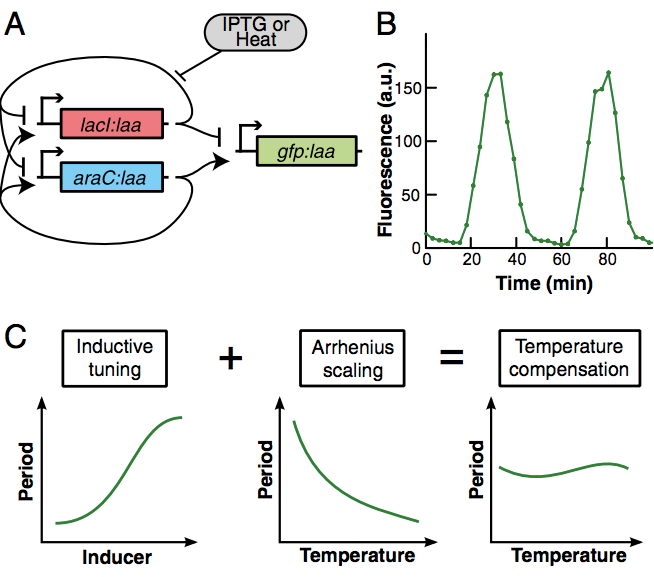
\includegraphics[width=0.8\textwidth]{stricker_tempcomp.png}
\end{center}
\begin{itemize}
\item Many temperature-sensitive LacI variants have been described, and combined with the ability to inhibit LacI through addition of lactose or its non-digestible analog IPTG, the hasty lab was able to find a regime where the change in LacI activity with temperature compensated the change in transcription and translation reaction rates. (Not perfectly, of course, but reasonably well.)
\end{itemize}
\begin{center}
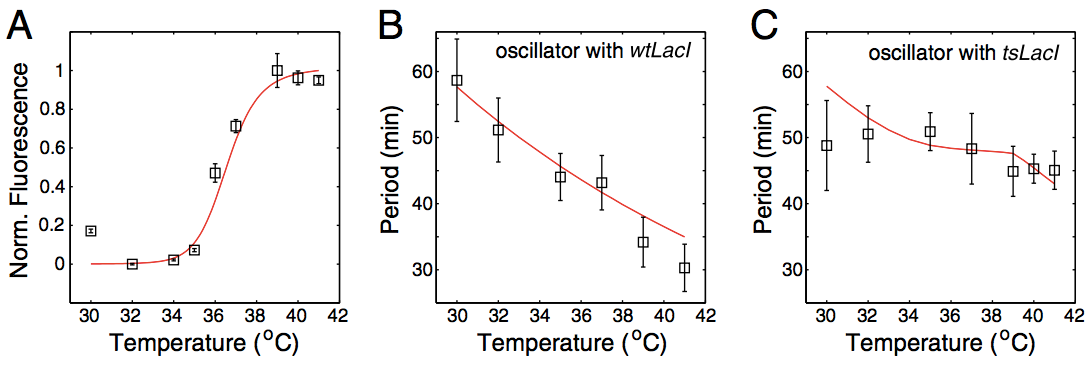
\includegraphics[width=0.8\textwidth]{hasty_tempcomp_results.png}
\end{center}

\section*{Quorum sensing}
\begin{itemize}
\item Another improvement introduced on the original system is coupling of oscillations between cells. Synthetic biologists often employ bacterial quorum sensing in situations that call for cell-to-cell communication, because they have relatively few moving parts and are well understood.
\item Bacterial quorum sensing is a means of cell-to-cell communication used to convey the simple message of how dense the population of cells is.
\item  Nowadays many biologists are familiar with quorum sensing as a means to decide whether enough bacteria are present that they can form a solid extracellular matrix through the secretion of protein or carbohydrate polymers. This type of extracellular matrix is called a \textit{biofilm}: it provides a solid adhesion point so that bacteria can enjoy the nutrient-rich environment in, e.g., a catheter tube without being swept away, and may make it more difficult to eradicate them through antibiotic treatment. The medical implications for preventing biofilm formation have made this an area of intensive study.
\item However, quorum sensing was discovered by Woody Hastings's group in the early 70s in another context entirely: the production of the photon-releasing enzyme luciferase by bioluminescent bacteria \textit{Vibrio fischeri} that live inside of the light organs of certain squids and fish.
\item The Hawaiian bobtail squid, for example, hides in sand by day and hunts at night, but is in turn prey to larger organisms that recognize it by the shadow it casts through the moonlight. Just as some jellyfish express blue and green fluorescent proteins, this squid has special organs for holding bioluminescent bacteria whose light obscures its shadow.
\item The squid dumps bacteria at dawn, retaining just enough that by the end of the day they will have reached a high enough density that they fluoresce through the night.
\item The \textit{Vibrio} quorum sensing system is based on a small molecule called acyl-homoserine lactone (AHL) that the bacteria produce using an enzyme called LuxI. Some of the AHL produced leaves the cell; the remainder may bind to a transcriptional activator called LuxR, causing it to become active and increase expression of LuxI as well as luciferase. Initially the majority of AHL is lost from the cell by diffusion, but when the cell density becomes high, AHL levels build externally and more AHL stays within the cell to promoter luciferase expression.
\end{itemize}

\section*{Oscillator coupling in the Hasty group model}
\begin{center}
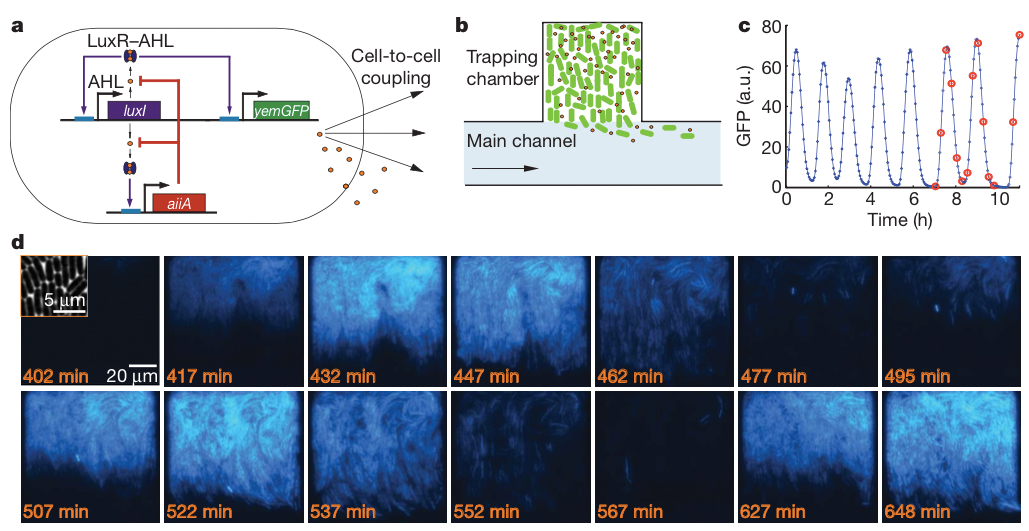
\includegraphics[width=0.7\textwidth]{danino_small.png}
\end{center}
\begin{itemize}
\item In 2010 (Danino et al.), the Hasty group created a modified version of their relaxation oscillator in which the promoters contained binding sites for LuxR-AHL. In place of AraC, LuxI was used as the activator (since it causes AHL to accumulate). The repressor was replaced by AiiA, an enzyme that breaks down AHL.  A fluorescent reporter, rather than luciferase, was used for the system's output.
\item The authors used specialized flow chambers to grow small communities of these cells, which they found fluoresced in coordinated fashion (if the group was small enough) and in waves when the chamber was very large. You will notice however that there is still variability in the period of the clock.
\end{itemize}
\begin{center}
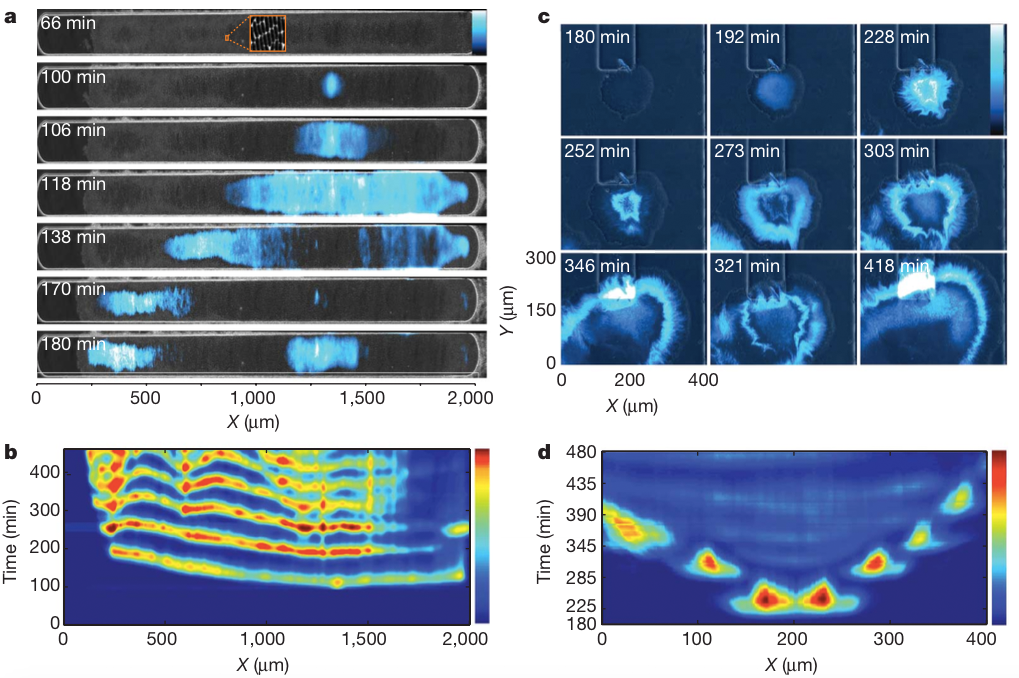
\includegraphics[width=0.7\textwidth]{danino_large.png}
\end{center}

\section*{Intrinsic vs. extrinsic noise}

\begin{itemize}
\item You have already heard in this course, at one point or another, that two identical promoters driving expression of nearly-identical reporters from different genomic loci will not necessarily have well-correlated expression. Michael Elowitz's classic results on intrinsic vs. extrinsic noise illustrate this point well.
\end{itemize}
\begin{center}
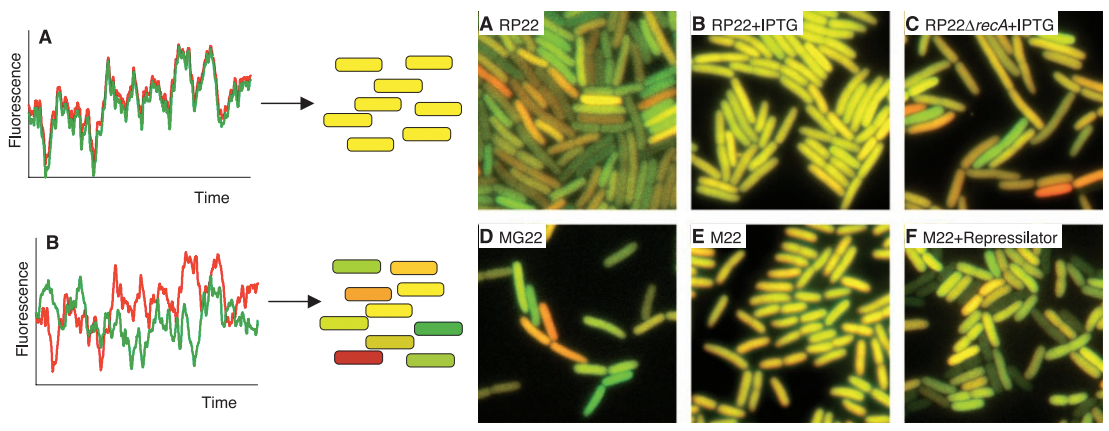
\includegraphics[width=\textwidth]{intrinsic_extrinsic.png}
\end{center}
\begin{itemize}
\item These experiments found intrinsic noise to be on par with extrinsic noise under many circumstances (particularly, when the promoter's rate of expression was not unusually large).
\item One may wonder what effect, then, placing \textit{luxI}, \textit{aiiA}, and GFP from separate loci might have on the oscillator's consistency. Although it may seem that the problem is resolved by placing all three ORFs in the same operon, in fact this is not ideal either, because the rate of expression for ORFs within an opeon is not identical but rather depends on gene order, RBS strength, etc.
\end{itemize}

\section*{Oscillator coupling through shared degradation machinery}
\begin{itemize}
\item Unfortunately this issue with coupling of production rates remains open. However, Prindle et al. (2014) have tackled the problem from the opposite end by improving coupling of degradation rates.
\item Returning to a strategy that the Hasty group had previously employed for the intracellular synthetic relaxation oscillator, Prindle and colleagues added the \textit{ssrA} degron to each protein in the circuit. (Recall that this had previously been performed with the motivation of increasing degradation rates.) As soon as one of ClpXP's substrates began to build up, all of the other substrates' degradation rates would slow down due to competition, and this would cause a synchronization in their accumulation and degradation -- a result they confirmed in vivo with a simple reporter system:
\end{itemize}
\begin{center}
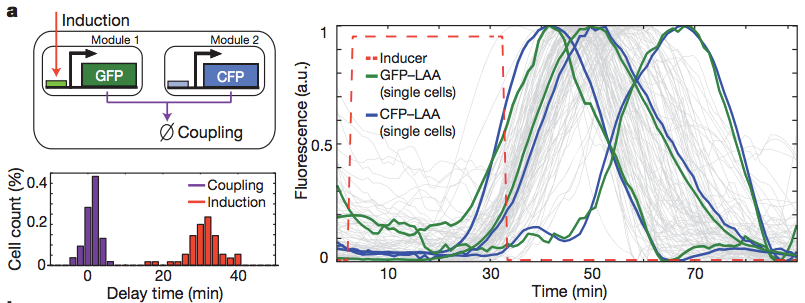
\includegraphics[width=0.6\textwidth]{prindle_reporter.png}
\end{center}
\begin{itemize}
\item Let us pause to reflect on the importance of controlled experiments in synthetic biology as elsewhere: the LAA tags have been a feature of these oscillators since 2008, but their potential contribution to coupling of protein levels was only elaborated quite recently!
\item Prindle et al. found that two clocks of radically-different period (the quorum sensing clock and intracellular negative autoregulation clock) could be synchronized to the same period and phase through saturation of ClpXP, even with nothing else to link them.
\end{itemize}
\begin{center}
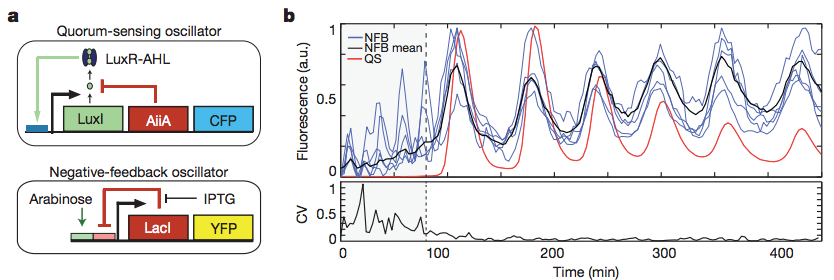
\includegraphics[width=0.7\textwidth]{prindle_clocks.png}
\end{center}
\begin{itemize}
\item The coupling was improved by placing even more load on ClpXP via hydrogen peroxide (which caused more proteins to be targeted for degradation). Ultimately the spread in amplitude and period of these clocks was much tighter than in the originals (image below).
\item We have seen that many features that improve the consistency of natural clocks can be implemented in synthetic systems with the predicted effects. (Not shown, for perceived time constraints, is an exploration of the clock's entrainment.) We have also begun to appreciate the importance of noise for the clock's deviation from ideal behavior -- a concept we'll explore in more detail in the following section of the course.
\end{itemize}
\begin{center}
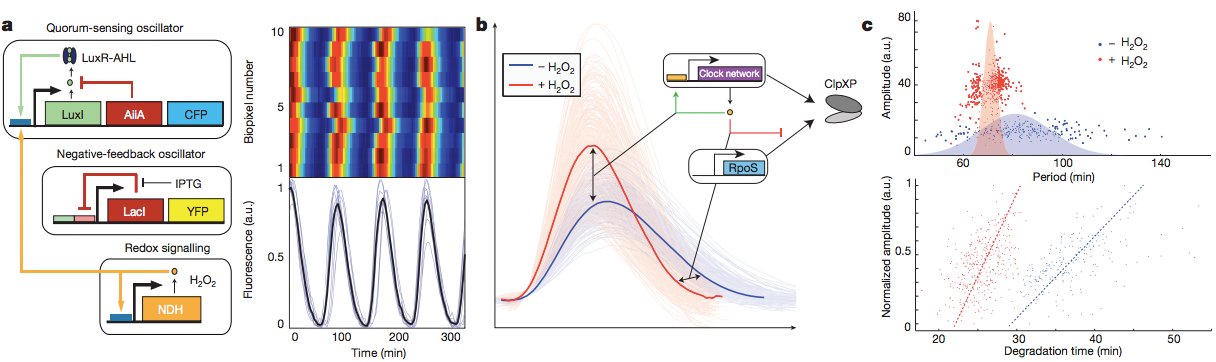
\includegraphics[width=\textwidth]{prindle_h2o2.png}
\end{center}

%\section*{Fruit fly circadian rhythms}
%
%\begin{itemize}
%\item The group of Albert Goldbeter (of zero-order ultrasensitivity fame) was the first to describe a dynamic model for a circadian clock in \textit{Drosophila melanogaster}, the fruit fly.
%\item Seymour Benzer's lab had identified several decades prior a series of mutants at the same \textit{per} (period) locus that either lacked circadian rhythm entirely or had clocks with a different period. (Flies walk around more during the subjective day-- particularly at dusk and dawn -- than during the subjective night; from traces of their motion we can discern the period of their clock.)
%\item The abundance of the protein encoded at this locus, PER, and its mRNA were found to oscillate with the same period as the flies' circadian clock. The mRNA's peak occurred about five hours before the protein's peak.
%\item The PER protein was known to be modified post-translationally by two separate phosphorylation events, both required for nuclear entry.
%\item In the nucleus, it binds to a transcriptional activator to inhibit it (the CLOCK/CYCLE complex). That transcriptional activator is needed for PER expression, so PER is effectively inhibiting its own transcription.
%\item An additional complication, not included in Goldbeter's model, is that the PER protein must be dimerized to Tim (Timeless) in order to avoid degradation. CLOCK/CYCLE inhibition also causes a decrease in \textit{tim} expression, further enhancing the loss of PER after nuclear entry.
%
%\end{itemize}
%
%\begin{center}
%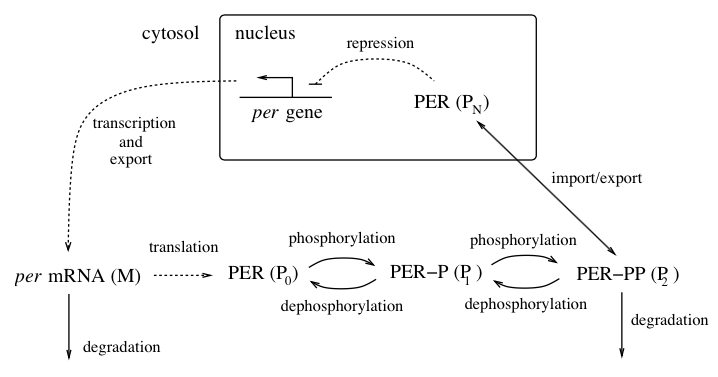
\includegraphics[width=0.7\textwidth]{goldbeter.png}
%\end{center}
%
%\begin{itemize}
%
%\item Leloup and Goldbeter's model focused on \textit{per} alone, using the following five species:
%
%\begin{eqnarray*}
%\frac{dm}{dt} & = & \frac{v_s}{1+ \left( \frac{p_n}{K_1} \right)^n} - \frac{v_m m}{K_{m1} + m}\\
%\frac{dp_0}{dt} & = & k_s m -  \frac{V_1 p_0}{K_{1} + p_0} +  \frac{V_2 p_1}{K_{2} + p_1}\\
%\frac{dp_1}{dt} & = & \frac{V_1 p_0}{K_{1} + p_0} -  \frac{V_2 p_1}{K_{2} + p_1} -  \frac{V_3 p_1}{K_{3} + p_1} +  \frac{V_4 p_2}{K_{4} + p_2}\\
%\frac{dp_2}{dt} & = &  \frac{V_3 p_1}{K_{3} + p_1} -  \frac{V_4 p_2}{K_{4} + p_2} - k_1 p_2 + k_2 p_N - \frac{v_d p_2}{K_d p_2}\\
%\frac{dp_n}{dt} & = & k_1 p_2 - k_2 p_N
%\end{eqnarray*}
%
%\item The parameters from this model were fit to generate oscillations. It was possible to choose them such that $n=1$ (i.e. PER was not required to dimerize); indeed the range of valid parameters for generating oscillations with period 24 hours was quite large.
%
%\item Although the parameters were chosen somewhat arbitrarily, Leloup and Goldbeter analyzed the effect of changing PER degradation rates ($v_d$) and found that this could cause the clock to oscillate with a variety of different periods. This fit well with the Benzer group's data on \textit{per} mutants.
%
%\end{itemize}

\end{document}